\subsubsection{Klassifikation} \label{grundlagen-klassifikation-0}

Ziel des Klassifizierungsschritts ist es, ein Klassifizierungsmodell zu trainieren, das in der Lage ist, Objekte in den Daten (dargestellt durch ihren Merkmalsvektor) in die entsprechende Klasse zuzuordnen. \\


% Splitting
Der Datensatz der Merkmalsvektoren, der im vorherigen Schritt des ERC erhalten wurde, wird in einen Trainingsset (engl. "training set") und einen Testset (engl. "testing set") unterteilt, so dass alle Klassen in beiden Sets vorhanden sind. Mit dem Trainingsdaten wird ein Klassifikator erstellt und trainiert. Der so erhaltene Klassifikator wird dann anhand der Daten des Testsets ausgewertet. Es ist wichtig, dass die Trainings- und Testsets unterschiedlich sind (d.h. nicht die gleichen im Daten Trainings- und Testset verwenden), da es sonst in einer {\"u}beranpassung (engl. "overfitting") des Klassifikator resultieren kann. Eine {\"u}berpassung tritt auf, wenn ein Klassifikator zuf{\"a}llige Schwankungen oder Rauschen in den Trainingsdaten "zu gut" lernt und dann bei neuen, unbekannten Daten deutlich schlechter abschneidet. Der Grund hierf{\"u}r ist, dass diese gelernten Schwankungen oder Rauschen in den Trainingsdaten keinerlei Relavanz f{\"u}r das eigentliche Klassifizierungsproblem haben. \\

\begin{figure}[h] \centering{
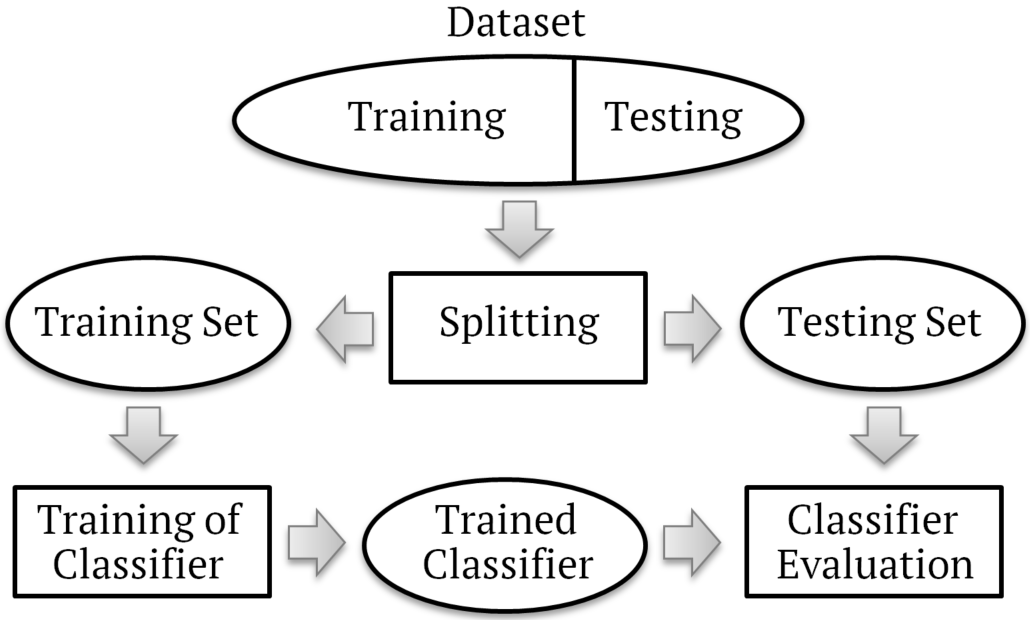
\includegraphics[width=12cm]{Images/splitting.png} 
\caption[Aufteilen eines Datensets in ein Trainings- und Testset]{Aufteilen eines Datensets in ein Trainings- und ein Testset. Das Trainingsset dient zum Erstellen und Trainieren eines Klassifikators. Die Performance wird mithilfe des Testsets ermittelt und bewertet. }}
\label{fig:splitting} \end{figure} \vspace{0.5cm}


% SVM
F{\"u}r die Klassifizierung wurde der state-of-the-art Klassifikator Support-Vector-Machine (SVM) verwendet.
SVM ist ein {\"u}berwachtes Lernansatz, der f{\"u}r bin{\"a}re Klassifikation oder Regressionszwecke genutzt werden kann. 
Das Ziel des SVM ist es eine Hyperebene (engl. "hyperplane") zu finden, die zwei Klassen im Raum der Merkmale trennt und gleichzeitig den Abstand (engl. "margin") zwischen der Hyperebene und den n{\"a}chsten Datenpunkten jeder Klasse maximiert.
F{\"u}r jeden Datenpunkt (dargestellt durch den entsprechenden Vektor von Merkmalen) den wir klassifizieren m{\"o}chten, wird ein Klassenettiket vergeben, je nachdem, zu welcher Seite der Hyperebene es geh{\"o}rt.
Die Methode hat ihren Namen von den "St{\"u}tzvektoren" (engl. "support vectors"), welche die n{\"a}chstgelegenen Vektoren beider Klassen zur trennenden Hyperebene sind. 
Cortes und Vapnik zeigten in \cite{svn1995}, dass die Gleichung der optimalen Hyperebene nur von diesen spezifischen Vektoren abh{\"a}ngig ist.
Abbildung \ref{fig:svm} zeigt eine optimale Hyperebene in 2D, die beide Klassen perfekt teilt.
Datenpunkte werden durch nicht-ausgef{\"u}llte blaue Dreiecke bzw. rote Kreise f{\"u}r beide Klassen dargestellt, w{\"a}hrend Unterst{\"u}tzungsvektoren durch ausgef{\"u}llte Punkte und Kreise hervorgehoben werden. \\

\begin{figure}[h] \centering{
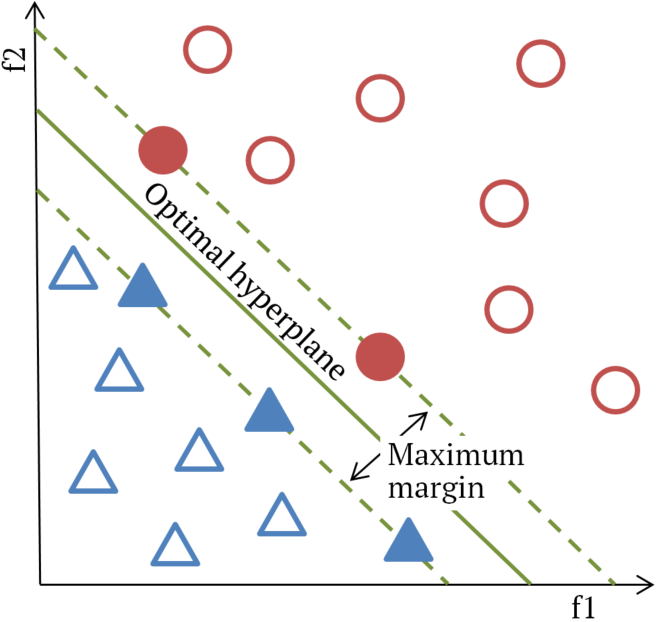
\includegraphics[width=8cm]{Images/svm.png} 
\caption[Beispiel eines SVM-Klassifikators im 2D Merkmalsraum]{Beispiel eines SVM-Klassifikators im zweidimensionalem Merkmalsraum: Die Datenpunkte beider Klassen (dargestellt durch nicht-ausgef{\"u}llte blaue Dreiecke und rote Kreise) sind durch eine Hyperebene getrennt, welche die Margin maximiert. St{\"u}tzvektoren werden als ausgef{\"u}llte Dreiecke und Kreise dargestellt. }}
\label{fig:svm} 
\end{figure} %\vspace{0.2cm}

Es ist anzumerken, dass SVM nur mit zwei Klassen funktioniert, aber sie k{\"o}nnen zu $ Z $ Klassen verallgemeinert werden.
Es gibt zwei Ans{\"a}tze zur Verallgemeinerung auf $ Z $ Klassen:
\begin{itemize} %[noitemsep]
  \item \underline{1 vs 1} besteht darin, Klassifikatoren f{\"u}r jedes Klassenpaar zu trainieren. Auf diese Weise werden $ Z(Z-1)/ 2$ Klassifikatoren trainiert, d.h. einen f{\"u}r jedes Klassenpaar.
  \item \underline{1 vs all} besteht darin, $ Z-1 $ Klassen als eine Klasse zu betrachten und die letzte als zweite Klasse anzunehmen, mit der der Klassifikator trainiert wird. Dies wird f{\"u}r jede Klasse wiederholt, was zu $ Z $ Klassifikatoren f{\"u}hrt, d.h. einen f{\"u}r jede Klasse. \\
\end{itemize}

% Kernel Trick
In der Praxis sind die Daten durch normales SVM fast nie linear trennbar.
Einer der Hauptgr{\"u}nde f{\"u}r die Beliebtheit von SVM ist jedoch die M{\"o}glichkeit es so genannten Kernel-Tricks.
Es basiert auf der Annahme, dass nicht-linear trennbare Daten linear trennbar werden k{\"o}nnen, wenn sie in einen Raum h{\"o}herer Dimension projiziert werden.
In \cite{svn1995} zeigten Cortes und Vapnik, dass die SVM-Klassifikationsentscheidungsfunktion als gewichtete Summe von Skalarprodukten zwischen St{\"u}tzvektoren und dem Vektor der zu klassifizierenden Merkmale ausgedr{\"u}ckt werden kann. 
Der Kernel-Trick nutzt dies aus, indem er eine Kernelfunktion einf{\"u}hrt, die ein skalares Produkt im hochdimensionalen Zielraum repr{\"a}sentiert. 
Diese Kernelfunktion er{\"u}brigt die eigentliche Zuordnung zwischen dem urspr{\"u}nglichen und dem hochdimensionalen Feature-Raum.
Au{\ss}erdem ist die Verwendung des Kernel-Tricks oft recheng{\"u}nstiger als andere Alternativen.
Die beiden beliebtesten Kernel sind der lineare und der Radial Basis Function (RBF) Kernel, definiert als: 
\begin{equation} 
\Large{ {\displaystyle K(\mathbf {x} ,\mathbf {x'} )=\exp \left(-\gamma{\|\mathbf {x} -\mathbf {x'}}\right\|)} }
\end{equation}
wobei $ x $ und $ x' $ Vektoren des Merkmalsraums bezeichnen und $ \gamma $ der Parameter ist, der die "Ausbreitung" (engl. "Spread") des Kernels definiert. \\


\begin{figure}[h] \centering{
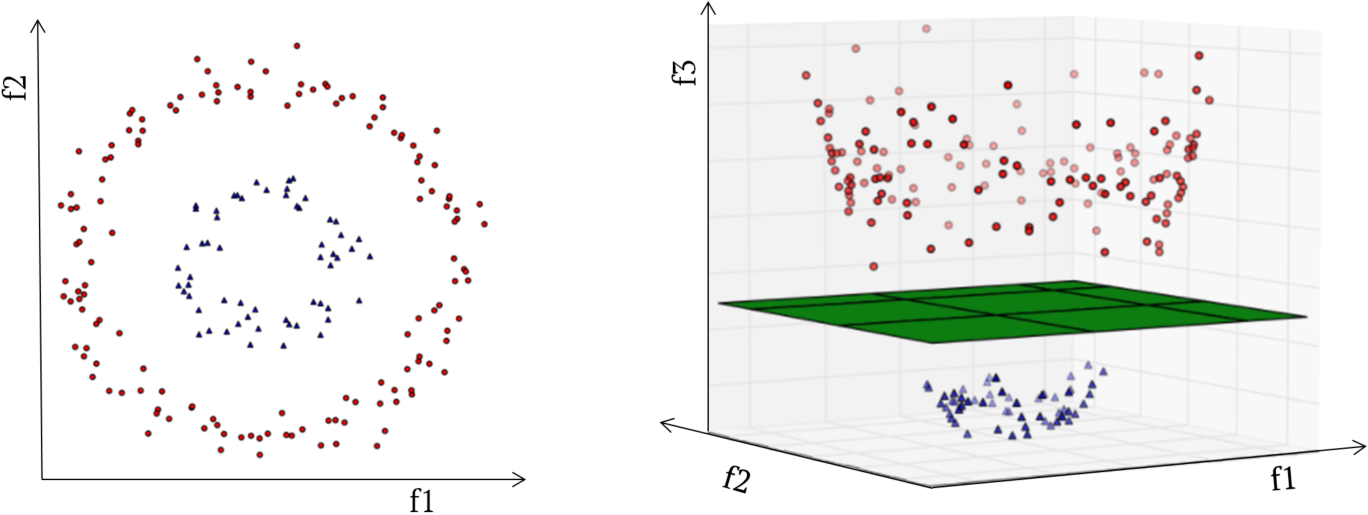
\includegraphics[width=\textwidth]{Images/kernel_trick.png} 
\vspace{-0.3cm} \caption[Beispiel f{\"u}r die Verwendung des Kernel-Tricks]{Beispiel f{\"u}r die Verwendung des Kernel-Tricks: Nicht-linear trennbare Daten in einem 2D-Merkmalsraum (links) k{\"o}nnen linear trennbar gemacht werden, wenn sie auf 3D projiziert werden (rechts) \cite{kernel_2013}.}}
\label{fig:kernel_trick} \end{figure} %\vspace{0.5cm}

% Overfitting
Normales SVM verwendet sogenannte hard-margins, die versuchen, eine optimale Hyperebene zu schaffen, die keine Fehlklassifizierungen zul{\"a}sst. 
Es ist jedoch oft besser, einige Klassifizierungsfehler zuzulassen, um eine {\"u}beranpassung zu verhindern und eine generalisierte Hyperebene zu erhalten. Diese allgemeinere Hyperebene liefert deutlich bessere und zuverl{\"a}ssigere Ergebnisse, wenn sie auf neue und unbekannte Datens{\"a}tze angewendet wird.
Hard-margin SVM kann zu einem Modell f{\"u}hren, das f{\"u}r die Trainingsdaten perfekt funktioniert, aber bei anderen Datens{\"a}tzen sehr schlecht, weil es seine Trainingsdaten "zu gut" gelernt hat.
Aus diesem Grund haben Cortes und Vapnik in \cite{svn1995} eine Variante des Standard-SVM-Klassifikators namens soft-margin SVM (oder auch C-SVM genannt) eingef{\"u}hrt, die eine Fehlklassifizierung von Beispielen beim Erstellen der trennenden Hyperebene toleriert.
Der soft-margin Parameter $C$ wird genutzt um die Anzahl der Fehlklassifikationen festzulegen.
Je gr{\"o}{\ss}er der Wert von $C$, desto weniger Fehleinstufungen sind zul{\"a}ssig.
Umgekehrt erlauben kleine Werte von $C$ mehr Fehlklassifizierungen, um die Verallgemeinerungsf{\"a}higkeit des Klassifikators zu verbessern. \\

\begin{figure}[h] \centering{
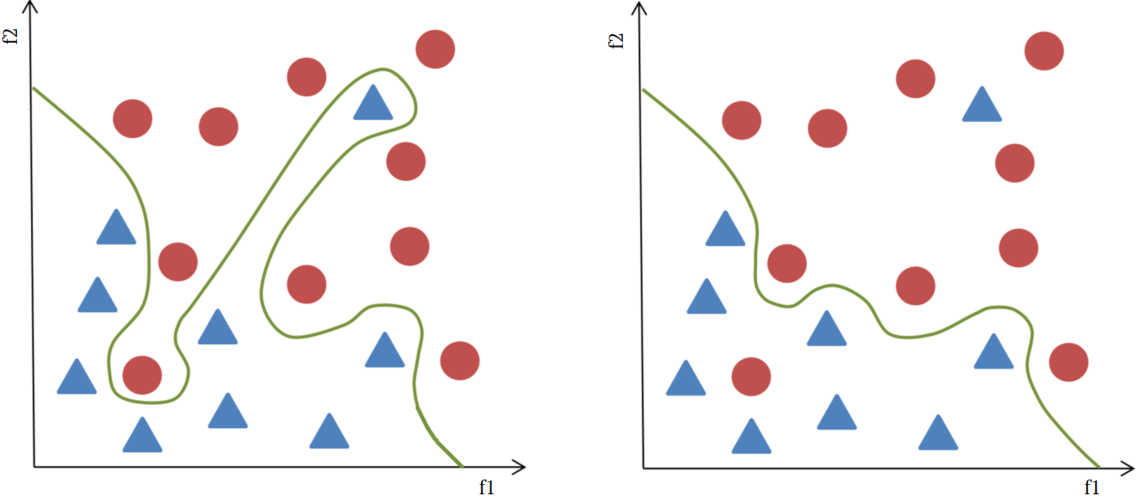
\includegraphics[width=\textwidth]{Images/overfitting.png} 
\vspace{-0.3cm} \caption[Beispiele f{\"u}r einen hard- und soft-margin SVM]{Beispiele f{\"u}r einen hard-margin SVM (links) und einen soft-margin SVM (rechts) in einem 2D-Merkmalsraum: Der hard-margin SVM trennt die beiden Klassen perfekt im Gegensatz zum Soft-Margin SVM, der einige Fehlklassifikationen zul{\"a}sst. }}
\label{fig:c-svm} \end{figure} 
%\vspace{0.5cm}